\section{Durchführung}
\label{sec:Durchführung}

\begin{figure}[H]
  \centering
  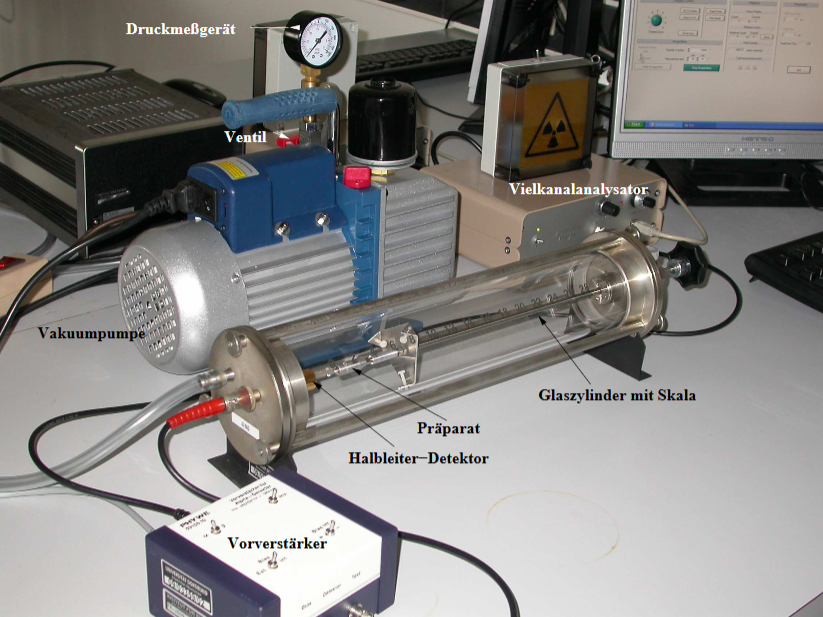
\includegraphics[height=8cm]{Aufbau.PNG}
  \caption{Aufbau der Messapparatur \cite{sample}.}
  \label{fig:aufbau}
\end{figure}

In Abbildung \ref{fig:aufbau} ist der Aufbau der verwendeten Messapparatur zu erkennen.
In einem Glaszylinder befindet sich eine Strahlungsquelle ($\alpha$-Strahlung) auf einer
beweglichen Schiene. Sie ist dabei in Richtung eines Halbleiter-Sperrschichtzählers am Ende
des Zylinders ausgerichtet.

Ein Halbleiter-Sperrschichtzähler besteht aus zwei aneinander liegenden Halbleiterplättchen,
zwischen denen sich eine Ladungsfreie Zone ausbildet. Angrenzend an die Ladungsfreie Zone liegen in den jeweiligen Plättchen
positiv und negativ geladene Zonen. Zudem kann aufgrund der Leitungseigenschaften
dieser Plättchen lediglich Strom in eine Richtung durch die Ladungsfreie Zone hindurchfließen. Legt man zudem eine Spannung
entgegen dieser Richtung ("Sperrrichtung") an, so vergrößert sich die Ladungsfreie Zone. Tritt nun ein ionisierendes
Teilchen in diese Zone ein, erzeugt dieses dort Elektronen-Loch-Paare. Diese werden durch das dort herrschende erlektrische Feld
getrennt und wandern zur entsprechend anders geladenen Zone. Durch diese Ladungsbewegung können letztendlich Stromimpulse gemessen werden,
welche natürlich Aufschluss auf die Anzahl der Zerfälle liefern.

Der Zähler ist wiederum über einen Verstärker und einen Vielkanalanalysator mit einem
Computer verbunden, auf welchem die gemessenen Zählraten graphisch dargestellt werden können.

Der Vielkanalanalysator "sortiert" dabei praktisch die gemessenen Stromimpulse nach ihrer Höhe.
Dies geschieht im wesentlichen durch einen Analog-Digital-Converter und einen Datenspeicher mit bestimmt vielen
Speicherplätzen (Kanälen). Der ADC wird beim eintreffen eines Impulses aktiv und bestimmt eine ganze Zahl, welche
dem der Impulsamplitude proportionalen Wert am nächsten kommt (dazu muss vorher ein Proportionalitätsfaktor eingestellt
werden). An dem der Zahl entsprechenden Speicherplatz wird zum dort vorhandenen Wert eine Eins addiert. Dadurch
kann am Ende der Messung dann überprüft werden, wie viele Impulse es mit Amplituden in einem bestimmten Bereich gab und man
kann sie wie beschrieben graphisch darstellen lassen.

Aus dem Glaszylinder kann dann noch die Luft mithilfe einer Vakuumpumpe evakuiert werden.

Zu Beginn des Versuchs wird die Strahlungsquelle bei normalem Luftdruck im Zylinder so weit
von dem Zähler entfernt, dass dieser gerade eben noch eine Strahlung misst. Außerdem wird
der Verstärker so angepasst, dass die gemessenen Zählraten trotz vorherrschendem Rauschen auf
dem Bildschirm des Computers gut sichtbar gemacht werden können. Sodann wird
der Zylinder evakuiert. Anschließend wird Stück für Stück wieder Luft hineingelassen.
Dabei werden jeweils bei unterschiedlichen Drücken (0-1000 mbar in 50 mbar Schritten)
über einen Zeitraum von 2 Minuten die Zählraten gemessen.
Danach wird eine analoge Messung mit einem leicht verringerten Abstand der Strahlungsquelle
zum Zähler durchgeführt.

Zum Schluss wird die Statistik des radioaktiven Zerfalls überprüft. Dafür wird der
Glaszylinder komplett evakuiert und die Strahlungsquelle wird verhältnismäßig weit vom
Zähler entfernt. Nun wird 100 mal über einen Zeitraum von jeweils zehn Sekunden die
Zählrate gemessen und die entsprechenden Werte vom Computer abgelesen.
